% DUET -- Evaluation (DAC 2027 draft, 2026-11-07). Text drafted 2026-11-07.
% Figures: tools/plot_eval.py -> results/paper_dac/fig_eval_{read,write,tput}.pdf, data in results/paper_dac/eval_data.csv.
% Bounded FTLs (DUET, DFTL, LeaFTL; uFTL dropped from the figures) = results/final_vbm. CoMap = results/final_comap_tune
% (tuned, comap_logfrac_ppm=990000 comap_p0=990000, 2026-11-08, was final_vbm: tput 0.46, WA 3.64, avg write 3.30). Page, FAST, IU+RMW = results/final_rp (traces, apps)
% and results/final_rp_a128 (raw I/O).
% Raw I/O: 4K:128K = 70:30 only, labelled by R:W (2026-11-06). Geomean over the 10 workloads, normalized to Page:
% throughput DUET 0.93, LeaFTL 0.73, DFTL 0.67, IU+RMW 0.66, FAST 0.57, CoMap 0.49.
% Avg. read DUET 1.03, FAST 1.51, IU+RMW 1.61, LeaFTL 1.65, CoMap 1.82, DFTL 2.41.
% Write metrics (WA, avg / p99 write) exclude the read-only YCSB-C (2026-11-08, READ_ONLY in plot_eval.py), 9 workloads:
% WA DUET 1.16, DFTL 1.06, LeaFTL 1.08, IU+RMW 2.36, FAST 2.62, CoMap 3.31.
% Avg. write DUET 1.11, DFTL 0.91, LeaFTL 1.15, IU+RMW 2.09, FAST 2.39, CoMap 3.06.
% p99 read DUET 1.02, FAST 1.35, IU+RMW 1.70, CoMap 1.71, DFTL 1.71, LeaFTL 2.10.
% p99 write DUET 1.06, DFTL 1.01, LeaFTL 0.86, IU+RMW 1.58, FAST 2.51, CoMap 3.46.
% FAST = FAST-B12 (same budget). FAST full (cache_bytes=1e9, results/final_fastfull, exceeds the budget in the worst case):
% tput 0.72, WA 1.33x, avg write 1.26, p99 write 1.03. TODO eval text: one sentence that FAST full still reaches only 72%.

\section{Evaluation}
\label{sec:eval}

% Setup facts: host Xeon Gold 6342, 408 GB DRAM, Ubuntu kernel 6.8.0. ssd_config.h SAMSUNG_970PRO base: 8 ch x 2 LUN,
% 32 KB flash page, read ~36 us, program 185 us, OP_AREA_PERCENT 0.07, 373 blocks. Device (logical) = SPFresh 21.6 GB,
% Alibaba 59.6 GB, apps 44.2 GB (memmap 44G), raw I/O 96.5 GB. Apps: ext4 + PostgreSQL (YCSB, BenchBase TPC-C) in
% dmapp.slice MemoryMax = 20% of the device = 8,830,058,496 B, MemoryHigh 7/8. Traces / raw I/O: trace_replay, QD 32.
% Alibaba = ali3: /mnt/nvme_mounted/alibaba_dwpd01to1.trace (8442.76 GiB writes), trace_prep sample=23/1000 region=1 MiB
% order=touch reads=1 -> 175.6 GiB writes, 70.7 GiB reads, 59.5 GB device, replayed fully (not truncated), warmup 0.5.
% Budget T = L*4/8 + NB*P/64 B (IU+RMW map + one valid bit per 32 KB IU) = 12.9% of L*4: 2.72 / 7.52 / 5.58 / 12.17 MB.
% Mapping reads and programs are counted in all WA and latency results (Section IV).
\subsection{Experimental Setup}
% (2026-11-11) One device for every workload (results/final_32g, results/nvmevirt/q_32g.sh): 32 GB host-visible
% (L = 8391056 pages), OP 7% of it, 274 superblocks of 128 MB = one 8 MB block (256 x 32 KB pages) per die x 16 dies.
% Budget T = L*4/8 + NB*P/64 = 4335816 B (tools/budget_vb.py 35073M 274); Page map L*4 = 33.6 MB = 32 MiB.
% Traces /mnt/nvme_mounted/dm_trace_32g: ali3 sample 13/1000 (kept 1.29% of 1 MB regions, 96.4 GiB writes, 40.0 GiB reads);
% SPFresh unsampled, untouched pages squeezed out (trace_prep region=4096 rtouch=1, address order): 26.9 GiB, 113.2 GiB
% writes, 2255 GiB reads (none dropped). Replayed up to the first 64 GiB of writes (1275 GiB reads), spfresh_full.csv kept.
% Raw I/O = tools/gen_synth_trace.py request lists replayed by tools/trace_replay (not fio: fio cannot align 4 KB and
% 128 KB requests each to its own size in one job). Memory cgroup 20% of the device = 6.4 GiB.
% Old (per-workload devices, 22--97 GB): kept in git history.
\textbf{Setup.} We run all experiments on a server with an Intel Xeon Gold 6342 CPU
and Linux kernel 6.8. The emulated SSD has eight channels with two dies each and
exposes 32\,GB to the host. Its OP space is 7\% of that capacity. All workloads and
FTLs use this device. We cap the mapping DRAM of
every FTL except the page-level mapping FTL at the DRAM of a uniform 32\,KB coarse IU,
an IU size used in production high-capacity SSDs~\cite{micron-iu,solidigm-csal},
which is 4\,MB. The page-level mapping FTL uses 32\,MB. DUET uses 64\,KB coarse IUs, so its coarse map takes half
of the budget and the fine map the other half.

\textbf{Workloads.} We run three types of workloads, synthetic raw I/O, real-world
traces, and applications. The synthetic raw I/O issues requests to the block device
directly, without a file system. The requests are uniformly random over the whole
device. Of the requests, 70\% are 4\,KB and 30\% are 128\,KB, each aligned to
its size, and the read ratio is 50\%, 70\%, or 90\%.
The real-world traces are the Alibaba cloud
block traces~\cite{alibaba-trace} and an I/O trace of SPFresh~\cite{spfresh}, a vector
search index with in-place updates. From the Alibaba traces, we take the volumes whose
drive writes per day are 0.1 to 1, which write 8.2\,TB in total. To fit them in the
32\,GB device, we keep 1.3\% of their address space by spatial
sampling~\cite{shards}, together with every request to the sampled space. We replay the
SPFresh trace without sampling until it writes 64\,GB, twice the device capacity,
which also reads 1.2\,TB. The raw I/O and the
traces run with 32 outstanding requests, and we measure the second half of each run.
The applications are YCSB
workloads A, B, and C~\cite{ycsb} and TPC-C~\cite{tpcc} on PostgreSQL and ext4,
each with 64 client threads. They run in a memory cgroup of 6.4\,GB, 20\% of the
device, which limits the page cache.

\textbf{Baselines.} We compare DUET with six other FTLs, which cover the three classes
of Section~\ref{sec:bg}. \textbf{Page} maps
every 4\,KB page and keeps the whole table in DRAM, without a DRAM limit.
\textbf{DFTL}~\cite{dftl} caches mapping entries in an LRU map cache and writes back the
dirty entries of a translation page together. \textbf{LeaFTL}~\cite{leaftl} learns linear
segments, each of which predicts the physical pages of consecutive LPNs, caches them
in DRAM, and sorts writes by LPN to form longer segments. \textbf{FAST}~\cite{fast} maps data blocks per NAND block and appends updates to one
sequential and several random log blocks, and we limit the number of log blocks so
that their page-level maps fit the DRAM budget. \textbf{CoMap}~\cite{comap} chooses page-level or
block-level mapping for each write request with a Q-learning agent. \textbf{CoarseIU}
maps all data with a uniform 32\,KB coarse IU and keeps the whole table in DRAM.
Small writes to the same coarse IU are merged in the 1\,MB write buffer, and a
partial coarse IU is written with RMW only when it leaves the buffer. Its
DRAM sets the budget that every other bounded FTL receives.

\begin{figure*}[t]
  \centering
  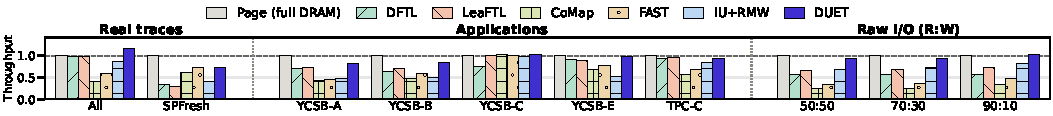
\includegraphics[width=\textwidth]{figs/fig_eval_tput.pdf}
  \vspace{-6.8mm}
  \caption{Throughput normalized to Page.}
  \label{fig:eval-tput}
  \vspace{-4.5mm}
\end{figure*}

% Numbers below: results/paper_dac/eval_data.csv (per workload) and the geomeans in the header comment.
\subsection{Read Latency}
Figure~\ref{fig:eval-read} shows the read path. DUET reads the mapping from NAND only
for spilled coarse IUs, so it needs 1.02 flash reads per host read on average and at
most 1.06, on SPFresh. DFTL and LeaFTL miss in their map caches and need up to 1.90
and 1.84 flash reads on SPFresh. As a result, the average read latency of DUET is
1.07$\times$ that of Page on average, whereas that of DFTL and LeaFTL is 2.51$\times$ and
1.75$\times$ that of Page.
% (2026-11-13) app averages from /sys/block stat (blklat.bt sector-keyed artifact, see tools/plot_eval.py). Was 0.91, 2.15, 1.58.
The average read latency of DUET is 34\%, 49\%, and 20\% lower than that of FAST,
CoMap, and CoarseIU on average. DUET writes small writes to fine
blocks without RMW and merges one coarse IU at a time, so its reads wait less behind
writes.
% (2026-11-12) geomean over 9 workloads (eval_data.csv), avg read / DUET: FAST 1.52, CoMap 2.09, CoarseIU 1.25. / Page: DUET 0.91, FAST 1.39, CoMap 1.91, CoarseIU 1.15.
% p99 read / Page: DUET 1.09, FAST 1.59, CoMap 2.00, CoarseIU 1.52. Was: 50:50 FAST 2.9x, CoMap 4.0x, YCSB-B CoarseIU p99 2.0x DUET.
The p99 read latency
shows a similar trend, and DUET has the lowest among the FTLs with
a limited DRAM budget.
% (2026-11-12) p99 read / Page geomean: DUET 1.09, CoarseIU 1.52, FAST 1.59, DFTL 1.77, CoMap 2.00, LeaFTL 2.04
% (avg: DUET 0.91, CoarseIU 1.15, FAST 1.39, LeaFTL 1.58, CoMap 1.91, DFTL 2.15). Was: DUET 1.09x, DFTL 1.77x, LeaFTL 2.04x of Page.
% SPFresh trace (dm_trace_sampled/spfresh.json): 100% 4K reads and writes, seq_frac 0.076, top 10% of 1 MB regions = 20% of writes, reads 20x writes.

\subsection{Write Amplification and Write Latency}
Figure~\ref{fig:eval-write} shows the write path. YCSB-C is read-only, so it is left
out. DUET writes small writes out of place as fine pages and merges them one coarse
IU at a time, so its WA stays close to that of Page, with a geometric mean of 1.28$\times$ Page. FAST and CoMap merge whole
blocks, and CoarseIU rewrites a 32\,KB unit for every smaller write. Their WA is
2.7$\times$, 3.6$\times$, and 2.2$\times$ that of Page on average.
% (2026-11-12) geomean WA / Page over 8 workloads (no YCSB-C): FAST 2.72, CoMap 3.59, CoarseIU 2.16, DUET 1.28.
% Was: FAST 3.0x, CoMap 4.1x on raw I/O, CoarseIU 9.3x on SPFresh.
As a result, the average write latency of CoarseIU, FAST, and CoMap is 2.1--3.6$\times$
that of Page, whereas that of DUET is 1.26$\times$. The p99 write
latency shows a similar trend.
% (2026-11-12) p99 write / Page geomean (8 workloads): DUET 1.29, CoarseIU 1.50, FAST 2.61, CoMap 3.74, DFTL 1.11, LeaFTL 0.93.
% Was: TPC-C p99 write of DUET 3.7x lower than FAST.
DFTL and LeaFTL also write out of
place at 4\,KB granularity and keep their write latency close to that of Page, but
they pay for it on the read path.
% avg write (excl. YCSB-C): DUET 1.11, IU+RMW 2.09, FAST 2.39, CoMap 3.06. p99 write DUET 1.06. TPC-C p99: FAST/DUET 4.6, IU+RMW/DUET 2.9.
% WA: CoarseIU 1.5x Page on synthetic raw I/O. DUET 1.9x Page on SPFresh.

On Alibaba, the WA of DUET is 14\% lower than that of Page. In this workload, small writes tend to be hot. DUET writes the
writes smaller than a coarse IU to fine blocks, apart from the coarse blocks, so it
separates hot data from cold data as data placement schemes
do~\cite{sepbit,midas,dogi}. Page writes all data to the same active block, so hot and
cold pages are mixed in a block and its GC copies more valid pages.

\subsection{Throughput}
Figure~\ref{fig:eval-tput} shows the throughput normalized to Page. DUET reaches 91\%
of the throughput of Page on average, whereas LeaFTL, CoarseIU, DFTL, FAST, and CoMap
reach 71\%, 70\%, 63\%, 56\%, and 45\%. On Alibaba, DUET is 16\% faster than Page
because its WA is 14\% lower. DUET is the slowest relative to
Page on YCSB-A and SPFresh, at 69\% and 78\%, where its WA is 1.4$\times$ and
2.4$\times$ that of Page and reads of spilled coarse IUs add mapping reads.

% (2026-11-12, user) mu-FTL paragraph removed from the paper. It was: under the same DRAM budget, 1.49 flash reads per host
% read, WA 4.0x Page, 33% of Page throughput (44 GB runs).
% uFTL (results/final_vbm, mu / mu_vb), geomean vs Page: tput 0.33, fr 1.49, avg read 3.58, p99 read 2.97,
% WA 4.05, avg write 1.87, p99 write 1.40 (write metrics excl. YCSB-C). tput Alibaba 0.11, SPFresh 0.17.

% Ablation: tools/plot_ablation.py -> results/paper_dac/fig_ablation.{pdf,png}, data in ablation_data.csv.
% (2026-11-12) 32 GB, five bars (user): Basic = nsfm (spill=0, fold_all=1, gc_select_cost=0), + GC decisions = ns (coarse-or-fine victim
% selection + copy-or-merge), + Cuckoo = nskl (ct_kick=500, DRAM timing 50 ns per visited bucket, 4 FTL cores; merge on a
% failed search), DUET = spill/load (main runs). results/final_32g/{ablation,kick_dram}. nsm (coarse-or-fine only) is in
% ablation_data.csv history: WA 16.2 YCSB-A, 19.7 YCSB-B, 45.3 SPFresh (over-merges without copy-or-merge).
\begin{figure}[t]
  \centering
  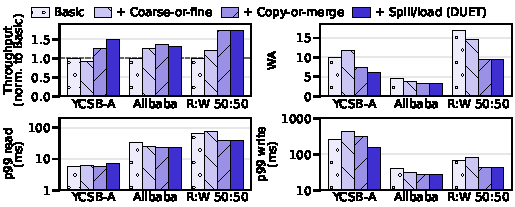
\includegraphics[width=\columnwidth]{figs/fig_ablation.pdf}
  \vspace{-6mm}
  \caption{Ablation. The two GC decisions are added to Basic one by one, and the two rightmost bars handle a full fine map by cuckoo hashing or by spill and load (DUET). Throughput is normalized to Basic.}
  \label{fig:eval-ablation}
  \vspace{-2.5mm}
\end{figure}

% Fine-area time series: tools/plot_ts.py -> results/paper_dac/fig_ts.{pdf,png} (results/final_32g/ts, q_32g_ab.sh, 5 s samples).
\begin{figure}[t]
  \centering
  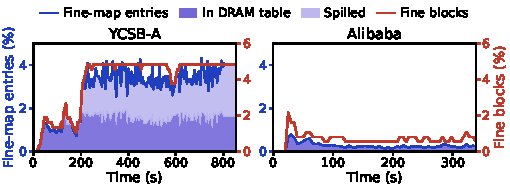
\includegraphics[width=\columnwidth]{figs/fig_ts.pdf}
  \vspace{-6mm}
  \caption{Fine-map entries, as a percentage of all logical pages, and fine blocks, as a percentage of all blocks, of DUET over time, sampled every 5\,s.}
  \label{fig:eval-ts}
  \vspace{-2.5mm}
\end{figure}

% Ablation numbers (2026-11-12): results/paper_dac/ablation_data.csv. WA Basic -> GC -> cuckoo -> DUET: YCSB-A 10.4 8.8 8.1 8.3,
% YCSB-B 9.8 8.6 7.7 7.4, Alibaba 4.8 3.6 3.6 3.6, 70:30 17.0 10.1 10.1 10.1. p99 read YCSB-A 6.4 11.4 8.4 ms (GC, cuckoo, DUET),
% YCSB-B 1.04 2.51 1.00 ms. p99 write YCSB-A 489 383 248 ms. Cuckoo YCSB-B: 6.05M searches, 1.23G probed buckets = 203 per
% search; YCSB-A 6.91M searches, 1.234G probes = 179 per search. Avg fine pages Basic / coarse-or-fine / copy-or-merge: YCSB-A 154K 39K 168K, YCSB-B 156K 38K 172K, Alibaba 41K 5.8K
% 23K, 70:30 94K 17K 38K (-75..-86% with coarse-or-fine). SPFresh (not shown): GC WA 16.4 -> DUET 13.3 (-19%), cuckoo tput 1.07 vs DUET 0.99 of Basic (+8%).
\subsection{Ablation Study}
Figure~\ref{fig:eval-ablation} adds the techniques of DUET to Basic on YCSB-A,
YCSB-B, Alibaba, and 70:30. Basic fills the fine blocks up to the fine-block cap, and its fine GC always
merges the fine pages of a victim into their coarse IUs. Coarse-or-fine victim selection shrinks the fine area,
which helps Alibaba and 70:30 but raises WA on YCSB-A and YCSB-B. There, a merge
copies the fine pages with the rest of their coarse IU, and new fine pages soon
invalidate part of it. The copy-or-merge decision improves this.
Together, the two decisions lower WA by up to 1.7$\times$ and raise the throughput
up to 1.61$\times$ that of Basic.

\emph{Cuckoo} makes room in full candidate buckets by moving entries along a path
to a free entry~\cite{cuckoo,bfscuckoo} and merges only when no path exists. It thus
merges less often than copy-or-merge and lowers WA by 8\% and 11\% on YCSB-A and
YCSB-B, where the fine map fills. Its search for a free entry on writes, however,
probes 179 and 203 buckets on average, which raises the p99 read latency by
1.8$\times$ and 2.4$\times$ and the p99 write latency on YCSB-B by 1.6$\times$.
DUET instead spills entries to NAND without searching and keeps the lower WA. Compared
with \emph{Cuckoo}, DUET lowers the p99 read latency by 27\% and 60\% and the p99
write latency by 35\% and 18\% on YCSB-A and YCSB-B.
% (2026-11-12) WA ns / ck / DUET: YCSB-A 8.78 8.12 8.29, YCSB-B 8.59 7.67 7.43 (ck -8%, -11% vs ns; DUET vs ck +2%, -3%).
% p99 read ns / ck / DUET: YCSB-A 6.38 11.42 8.37, YCSB-B 1.04 2.51 1.00 ms. p99 write: YCSB-A 489 383 248, YCSB-B 163 262 215 ms
% (ck p99 write is lower than ns on YCSB-A, so only YCSB-B is cited). Alibaba and 70:30: the three bars are within 1%.
% YCSB-A merge WA (fold) 0.33 (ns) vs 0.17 (DUET). Write queue in the measured half 261 vs 132 in flight at 165 vs
% 169 MB/s. YCSB-B is the other way (fold 0.37 vs 0.10 but p99 write 163 vs 215 ms), not written.

\subsection{Fine-Area Size over Time}
Figure~\ref{fig:eval-ts} shows how the fine area of DUET changes over time. Fine-map
entries are shown as a percentage of all logical pages. The fine area grows and
shrinks differently in each workload. On SPFresh, all writes are smaller than a
coarse IU, so the fine blocks stay at their limit, 4.0\% of all blocks, and fine-map
entries stay at 2.7--3.1\% of the logical pages. On Alibaba, 79\% of the written data
comes in writes of 64\,KB or larger, so the fine area stays smaller. It peaks early
in the run at 1.8\% of all blocks and 0.8\% of the logical pages, and then shrinks to
0.7--1.1\% of all blocks and 0.2--0.4\% of the logical pages. In both workloads,
spilled entries stay within 1.4\% of the logical pages, and Alibaba spills none.
% (2026-11-12) write sizes from /mnt/nvme_mounted/dm_trace_32g: spfresh.csv 100% of writes < 64 KB. ali3.csv 93.1% of
% write requests < 64 KB but 79.4% of written bytes in requests >= 64 KB.
% (2026-11-12) 32 GB, results/final_32g/ts (proposedst_g32), NB = 274: limit 11 = 4.0%, SPFresh after the first third
% fpages 2.66--3.12% of L, spages up to 1.42%. Alibaba peak 5 blocks = 1.8%, 0.79% of L, then 2--3 blocks, 0.15--0.44%.
% (2026-11-11, 44 GB) was YCSB-A + Alibaba: limit 18 = 4.8% of NB 373, YCSB-A spilled 2.6%, Alibaba peak 8 = 2.1%.
% (2026-11-08) was: 278K spilled entries (YCSB-A), 114K peak and 30--40K (Alibaba).

% Coarse-IU sensitivity (2026-11-09): results/final_usens (q_usens.sh), U=16 = final_vbm. tools/usens_table.py ->
% results/paper_dac/usens_data.csv, tools/plot_usens.py -> fig_usens. Same map_budget_ppm, so a larger U leaves more DRAM
% to the fine table. Geomean tput / Page: 0.91 0.92 0.87 0.86 (64/128/256/512 KB), WA 1.22 1.25 1.36 1.36.
% SPFresh: flash reads per host read 1.14 -> 1.06 -> 1.03 -> 1.02, tput 0.73 0.82 0.86 0.86. 70:30: tput 0.95 0.94 0.66 0.64,
% WA 1.10 1.11 1.63 1.69. YCSB-A WA 1.33 -> 1.43, TPC-C 1.14 -> 1.29.
\begin{figure}[t]
  \centering
  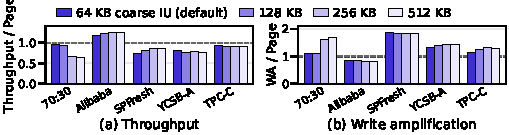
\includegraphics[width=\columnwidth]{figs/fig_usens.pdf}
  \vspace{-6mm}
  \caption{DUET with coarse IUs of 64--512\,KB under the same DRAM budget, normalized to Page.}
  \label{fig:eval-usens}
  \vspace{-2.5mm}
\end{figure}

\subsection{Coarse-IU Size}
Figure~\ref{fig:eval-usens} varies the coarse IU of DUET from 64\,KB to 512\,KB under
the same DRAM budget. A larger coarse IU shrinks the coarse map and leaves more
DRAM to the fine map, so fewer fine-map entries spill. On SPFresh, the flash reads
per host read drop from 1.06 to 1.00, and the throughput rises from 78\% to up to
84\% of Page. A larger coarse IU, however, turns more writes into fine pages. On
70:30, the 128\,KB writes still cover a 128\,KB coarse IU, but
become fine pages from 256\,KB on. Its WA rises from 1.1$\times$ to
1.9$\times$ that of Page, and its throughput drops from 93\% to 57\%. On YCSB-A,
YCSB-B, and TPC-C, the throughput changes by less than 4\% across the four sizes.
The coarse IU thus works best when it is no larger than the large writes of the workload.
% (2026-11-12, 32 GB, results/final_32g/usens, q_32g_ab.sh) usens_data.csv U=16/32/64/128: 70:30 tput 0.93/0.94/0.61/0.57,
% WA 1.13/1.11/1.76/1.90. SPFresh fr 1.06/1.01/1.00/1.00, tput 0.78/0.83/0.84/0.82. YCSB-A tput 0.69/0.69/0.70/0.71,
% YCSB-B 0.90/0.90/0.93/0.90, TPC-C 0.92/0.89/0.89/0.90.
% removed 2026-11-10 (geomean no longer in Fig. 10): Over the five workloads, the throughput of DUET stays at 86--92% of Page
